		\chapter{Begriffe \& Definitionen}

\begin{description}
	\item[Schwingung] eine sich zeitlich periodisch wiederholende Änderung einer oder mehrerer physikalischer Größen um enen Mittelwert
	\item[Elongation] Auslenkung -- Entfernung von einer Ruhelage zu einem Zeitpunkt \(s(t)\)\index{Elongation}
	\item[Amplitude] Betrag der maximalen Auslenkung \(\hat{s}\)\index{Amplitude}
	\item[Periode(ndauer)] die Dauer einer Vollständigen Schwingung \(T\)
	\item[Frequenz] Anzahl von Schwingungen pro Zeit \(f = \frac{1}{T}\)\index{Frequenz}
	\item[Winkelgeschwindigkeit] Drehung im Bogenmaß je Zeit \(\omega = \dot{\varphi} = 2 \cdot \pi \cdot f\)\index{Winkelgeschwindigkeit}
	\item[Rückstellkraft] Kraft die da Pendel in Richtung der Ruhelage beschleunigt \(F_R\)\index{Rückstellkraft}
	\item[Harmonische Schwingung] eine Schwingung, deren \(t\)-\(s(t)\)-Diagramm sinusförmig ist, wobei \(F_R \sim s(t)\) gilt \index{Harmonische Schwingung}
\end{description}


				\chapter{Harmonische Schwingung}

		\section{allgemeiner Lösungsansatz}

Im Allgemeinen hat sich bei uns der Lösungsansatz etabliert, eine Differentialgleichung zweiten Grades\index{Differentialgleichung} aufzustellen. Dabei wird die Rückstellkraft \(F_R\) auf zwei verschiedene Arten ausgerechnet. Einmal über den Zusammenhang \(F_R = m \cdot a(t)\) und das andere mal über den Zusammenhang \(F_R = - D \cdot s(t)\). Zur Diffenentialgleichung wird die Gleichung dann, weil \(\dot{s}(t) = v(t)\) und \(\dot{v}(t) = a(t)\) und somit \(\ddot{s}(t) = a(t)\). Unser Lösungsansatz ist also im Allgemeinen

	\begin{equation}
	m \cdot \ddot{s}(t) = - D \cdot s(t)
		\label{loesungsansatz}
	\end{equation}
	Die Lösung dieser Gleichung ist dann für uns die \textit{Sinusfunktion}, da
    sie diejenige Funktion ist, die ihrer zweiten Ableitung proportional
    ist\footnote{\(f(x) = \sin(x) ~~ f''(x) = - \sin(x)  ~~ f(x) = - f''(x)\)}. Mit ihr ergibt sich
	\begin{eqnarray}
		s(t) & = & \hat{s} \cdot sin(\omega \cdot t + \varphi) 
			\label{s(t)} \\
		\dot{s}(t) & = & \hat{s} \cdot \omega \cdot cos(\omega \cdot t + \varphi ) \\
		\ddot{s}(t) & = & - \hat{s} \cdot \omega^2 \cdot sin(\omega \cdot t + \varphi)
			\label{a(t)}
	\end{eqnarray}
Mit diesen Gleichungen lässt sich eine harmonische Schwingung beschreiben\footnote{\(\varphi\) ist die Phasenverschiebung}\index{Phasenverschiebung}. Als nachgewiesen, dass es sich bei der Schwingung um eine harmonische Schwingung handelt, gilt es, wenn man zeigen kann, dass
	\begin{eqnarray}
		F_R(t) &=& - D \cdot s(t) 
			\label{F sim s}\\
		D &=& m \cdot \omega^2
	\end{eqnarray}
 für die \emph{komplette} Schwingung gilt.


Setzt man nun Formel \ref{s(t)} und Formel \ref{a(t)} in Formel \ref{loesungsansatz} ein, so ergibt sich\footnote{mit \(\omega = \frac{2 \cdot \pi}{T}\)} für die Periodendauer \(T\) einer periodischen Schwingung allgemein

	\begin{equation}
		T = 2 \cdot \pi \cdot \sqrt{\frac{m}{D}}
			\label{T}
	\end{equation}

		
		
		
		
		\section{Das Fadenpendel}


Bei einem Fadenpendel\index{Fadenpendel} wirkt bei einer Masse immer eine Kraft
\(F_A\) in der Verlängerung des Fadens. Sie ist die Reactio der Zentripetalkraft
\(F_Z\), die den Schwingkörper auf seiner Kreisbahn hält. Zusätzlich greift
jederzeit die Schwerkraft \(F_g\) am Schwingkörper an. Mithilfe eines
Kräfteparallelogramms kann man die Schwerkraft nun zerlegen und erhält
einerseits \(F_A\), andererseits die Rückstellkraft \(F_R\). Diese
weist\footnote{so sie existiert -- im Ruhepunkt nämlich nicht} immer tangential zur Kreisbahn in Richtung der Ruhelage.


	\begin{figure}[h]
		\centering
		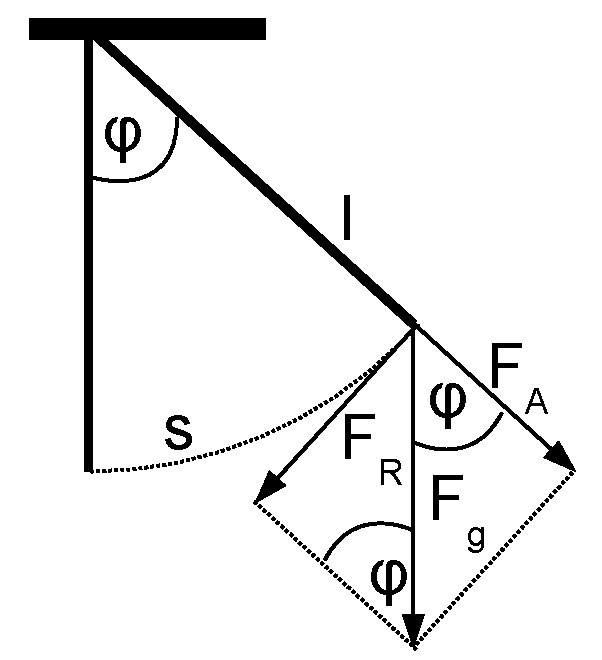
\includegraphics[width=0.35\textwidth]{mat/federpendel}
		\caption{Skizze eines Federpendels mit den bedeutenden Größen eingetragen}
			\label{skizze_federpendel}
	\end{figure}
Vom Nebenwinkelsatz aus kann man den Auslenkungswinkel \(\varphi\) noch an verschiedenen Stellen finden. Hier gelten dann die Beziehungen am rechtwinkligen Dreieck

	\begin{equation}
		\frac{F_R}{F_g} = sin(\varphi) 
			\label{F_R}
	\end{equation}
Der Winkel \(\varphi\) (im Bogenmaß) wiederum ist definiert mit 

	\begin{equation}
		\varphi = \frac{s}{l}
			\label{sinusnaehrung}
	\end{equation}
Für kleine Winkel \(\varphi\) gilt nun \(\varphi \approx sin(\varphi)\). Führt man diese Nährung jetzt entweder bei Formel \ref{F_R} oder bei Formel \ref{sinusnaehrung} durch, so erkennt man, dass

	\begin{equation}
		\frac{F_R}{F_g} \approx \frac{s}{l} ~~ \Rightarrow ~~ F_R \approx \frac{F_g}{l} \cdot s
			\label{naehrungsgleichung}
	\end{equation}
Da sowohl \(F_g = m \cdot g\) als auch \(l\) konstant sind, hängt \(F_R\) bei einer Schwingung nur von \(s\) ab. Damit ist also bewiesen, dass das Fadenpendel für kleine Auslenkungen \(\varphi < 6\)\textsuperscript{o} eine \emph{harmonische Schwingung} ausführt. Seine Richtgröße ist 

	\begin{equation}
		D = \frac{m \cdot g}{l}
			\label{richtgroesse_fadenpendel}
	\end{equation}
		
		
		
		\section{Das Federpendel}
	

Bei einem Federpendel hängt an einer Feder mit der Federhärte \(D\) ein Schwingkörper der Masse \(m\). Die Ruhelage dieses Systems ist dann erreicht, wenn die Kraft, mit der die Feder am Schwingkörper zieht \(F_F\) so groß ist, wie der Schwerkraft \(F_g\). Da bei einer Feder das \textsc{Hook}'sche Gesetz \(D = \frac{F}{s}\) gilt, gilt weiter

	\begin{equation}
		F_F = D \cdot s = - F_g ~~ \Rightarrow ~~ s_0 = - \frac{m \cdot g}{D}
			\label{s_0}
	\end{equation}
\(s_0\) ist dabei die Auslenkung des Pendels vom völlig unausgelenkten Zustand der Feder aus.

Das \textsc{Hook}'sche Gesetz\index{Hook'sches Gesetz} macht hier von Anfang an klar, dass es sich bei der Schwingung um eine harmonische handelt. Die Federhärte entspricht der Richtgröße\footnote{beide heißen deshalb \(D\)}. Besteht ein System aus einem Schwingkörper zwischen zwei Federn, so gilt für die Richtgröße
\begin{equation}
	D = D_1 + D_2
\end{equation}
		
	
	
		\section{Das Wasserpendel}

Ein Wasserpendel\index{Wasserpendel} besteht aus einem U-Rohr mit dem konstanten Querschnitt \(A\) in das Wasser der Masse \(m_{ges}\) mit der Dichte \(\varrho\) gefüllt wird. Die Wasseroberflächen in den beiden Rohrteilen stehen einander gegenüber und die Wassersäule hat insgesamt die Höhe \(2 \cdot h_0\), weil \(h_0\) die (gebogene) Strecke vom unteren Rohrmittelpunkt bis zu einem der Wasserspiegel ist. Die Schwingung mit der Elongation \(s(t)\) schwingt um diesen Pegelstand\footnote{\(h(t) = h_0 + s(t)\)}.


Wird nun das Wasser auf Seite A um \(s^{+}\) ausgelenkt, so sinkt der Pegel auf Seite B um \(- s^{+}\). Die Wassersäule ist auf Seite A \(2 \cdot s^{+}\) höher. Dieses \textit{Mehr} an Wasser \(V^{+}\) erfährt nun die Gewichtskraft \(F_g = m^{+} \cdot g\) nach unten, die gleichzeitig als Rüchstellkraft \(F_R\) fungiert. Über die Zusammenhänge von Masse, Dichte und Volumen (\(m = \varrho \cdot V\)) und der Umrechnung des Volumens (\(V^{+} = A \cdot 2 \cdot s^{+}\)) ergibt sich so für die Rückstellkraft
	
	\begin{equation}
		F_R = g \cdot \varrho \cdot A \cdot 2 \cdot s^{+}
			\label{rueckstellkraft_wsserpendel}
	\end{equation}
Dabei sind außer \(s^{+}\) alles Konstanten. Es ergibt sich für das Wasserpendel also eine Richtgröße \(D\) \index{Richtgröße} von

	\begin{equation}
		D = 2 \cdot g \cdot \varrho \cdot A
			\label{richtgroesse_wasserpendel}
	\end{equation}




		\section{Der Schwingkreis}


Ein Schwingkreis\index{Schwingkreis} ist ein Stromkreis, der im einfachsten Falle lediglich einen Kondensator\index{Kondensator} der Kapazität \(C\) und eine Spule\index{Spule} der Induktivität\index{Induktivität} \(L\) enthält. In ihm schwingt Strom der Ladung \(Q\) zwischen Kondensator und Spule hin und her. Aufgrund des simplen Aufbaus\footnote{Die Spannung des Kondensators \(U_C\) liegt direkt an der Spule an, ebenso wie die Induktionsspannung \(U_{ind}\) direkt am Kondensator anliegt} gilt im Stromkreis

	\begin{eqnarray}
		U_{ind} &=& - L \cdot \dot{I}(t) = - L \cdot \ddot{Q}(t)
			\label{U_spule} \\
		U_C &=& \frac{Q(t)}{C} = \frac{1}{C} \cdot Q(t)
			\label{U_kondensator} \\
		U_C &=& U_{ind} 
			\label{U = U}
	\end{eqnarray}
Der Kondensator wird anfangs einmalig geladen. Somit steckt im Kondensator
Energie \(E_{el}\). Der Kondensator entlädt sich nun langsam über die Spule,
dabei fließt logischerweise Strom -- und zwar mehr Strom, als zu dem Zeitpunkt
da der Kondensator noch ungeladen war -- somit steigt \(\dot{I}(t)\). Es ergibt
sich nach den Gleichungen \ref{U_spule} und \ref{U = U} eine
Induktionsspannung.\index{Induktionsspannung}\index{Lenz'sche Regel} Diese wirkt
dem Stromfluss entgegen (Siehe Kap. \ref{kap_lenzsche_regel} auf S.
\pageref{kap_lenzsche_regel}) und damit kann sich der Kondensator nicht sofort
entladen. Der Entladestrom nähert sich nun langsam (asymptotisch) seinem Maximum
an. 

In der Zeit, in der der Kondensator entladen wurde, baute sich in der Spule (und rundherum) ein Magnetfeld auf. Dieses Magnetfeld speichert nun die Energie \(E_{mag}\), die der Kondensator vorher enthalten hatte (\(E_{el} = E_{mag}\)). Wenn der Kondensator schließlich leer ist, ergibt sich erneut eine Induktionsspannung. Da der Strom vorher einen relativ großen Wert hatte und nun völlig "`abgeschaltet"' ist, wird \(\dot{I}(t)\) infolgedessen stark negativ und es wird erneut Spannung induziert, die den bereits abgebrochenen Stromfluss weiter unterhält.

Durch diese Induktionsspannung wird der Kondensator nun wieder geladen. Wenn das Magnetfeld komplett abgebaut ist, wird der Kondensator wieder so viel Energie haben, wie direkt nach dem Aufladen\footnote{von Verlusten der Dämpfung sei hier abgesehen}. Die Platte, die vorher aber negativ war, ist jetzt positiv und anderstherum. Das E-Feld hat sich also umgekehrt. Wenn der Vorgang dann wieder von Vorne beginnt, wird auch das B-Feld der Spule in die andere Richtung weisen als zuvor.

Es handelt sich hierbei um eine harmonische Schwingung, bei der Stromstärke und Spannug einer Sinusfunktion folgen. Setzt man die Gleichungen \ref{U_spule} und \ref{U_kondensator} in Gleichung \ref{U = U} ein, so erhält man eine Differentialgleichung \(\ddot{Q}(t) = - \frac{1}{L \cdot C} \cdot Q(t)\) deren Lösung wieder eine Sinusfunktion ist:\index{Differenzialgleichung}
	\begin{eqnarray}
		Q(t) &=& \hat{Q} \cdot cos(\omega \cdot t)
			\label{schwingkreis_Q} \\
		I(t) &=& - \hat{I} \cdot sin(\omega \cdot t)  = - \frac{\hat{Q}}{\sqrt{L \cdot C}} \cdot sin(\omega \cdot t) \\
		U(t) &=& \hat{U} \cdot cos(\omega \cdot t)
	\end{eqnarray}
Für den Schwingkreis ergibt sich eine Periodendauer von
	\begin{equation}
		T = 2 \cdot \pi \cdot \sqrt{L \cdot C}
	\end{equation}
Will man mechanische und elektrische Schwingungen Vergleichen, so gelte folgende Entsprechungen:
	\begin{eqnarray*}
	s 	& \widehat{=} & Q \\
	v 	& \widehat{=} & I \\
	a & \widehat{=} & \dot{I} \\
	D & \widehat{=} & \frac{1}{C} \\
	m & \widehat{=} & L \\
	\frac{1}{2} \cdot D \cdot s^2 & \widehat{=} & \frac{1}{2} \cdot  \frac{1}{C} \cdot  Q^2 \\
	\frac{1}{2}  \cdot m  \cdot v^2 	& \widehat{=} & \frac{1}{2}  \cdot L  \cdot I^2 
	\end{eqnarray*}


				\chapter{Gedämpfte Schwingungen}

\index{Gedämpfte Schwingung}Im Gegensatz zur idealen harmonischen Schwingung nimmt die Amplitude\index{Amplitude} \(\hat{s}\) im Laufe der Schwingung ab. Energie der Schwingung wird in andere Energieformen umgewandelt. Dies geschieht im Allgemeinen durch Kräfte \(F_{gl}\) die aus der Reibung schwingender Systeme resultieren. 

	\section{Konstante Reibung} 
Konstante Reibung tritt bspw. bei mechanischen Schwingungn auf. Hierbei ist die Bremsende Kraft \(F_{gl}\) konstant. Es gilt also für die Rückstellkraft \(F_R\)
	\begin{equation}
		F_R = m \cdot \ddot{s}(t) = - D \cdot s(t) - F_{gl}
	\end{equation}
Es gilt also hier das lineare Kraftgesetz nicht mehr und somit handelt es sich nicht um eine harmonische Schwingung. Die Amplitude \(\hat{s}\) der Schwingung nimmt bei jeder Schwingung \textit{linear} um \(s^{-}\) ab, mit
	\begin{equation}
		s^{-} = \frac{2 \cdot F_{gl}}{D}
	\end{equation}
	
	
	\section{Reibung abhängig von der Geschwindigkeit} 
Geschwindigkeitsabhängige Reibung tritt beispielsweise bei der Wirbelstrombremse\index{Wirbelstrombremse} auf. Hierbei nimmt die Amplitude \(\hat{s}\) zwischen den einzelnen Schwingungen exponentiell ab. Für die Rückstellungskraft ergibt sich hierbei
	\begin{equation}
		F_R = m \cdot \ddot{s}(t) = - D \cdot s(t) - R \cdot \dot{s}(t)
	\end{equation}
\(R\) ist hierbei eine Reibungskonstante. Auch hier liegt keine harmonische Schwingung vor. Eine Lösung der Differentialgleichung\footnote{\(m \cdot \ddot{s}(t) = - D \cdot s(t) - R \cdot \dot{s}(t)\)} ist hierbei die Funktion
	\begin{equation}
		s(t) = \hat{s} \cdot e^{- k \cdot t} \cdot sin(\omega \cdot t)
	\end{equation}
wobei \(\omega\) von der Eigenfrequenz\footnote{also der Frequenz, die das System ohne Reibung ausführen würde}  \(\omega_0\) abweicht. Hier gilt
	\begin{equation}
		\omega = \sqrt{\omega_0^2 - k^2}
	\end{equation}
Wobei auch \(k\) eine Reibungskonstante ist mit \(k = \frac{R}{2 \cdot m}\).

Bei dieser Art der Schwingungen muss man zwischen drei verschiedenen Sorten unterscheiden:
	
\begin{description}
	\item[Schwingfall]\index{Schwingfall} \(\omega_0 > k^2\) Das System Schwingt und die Amplitude nimmt exponentiell ab
	\item[Aperiodischer Grenzfall]\index{Aperiodischer Grenzfall} \(\omega_0 = k^2\) Das System schwingt fast eine halbe Periode lange, die Amplitude geht jedoch in kürzestmöglicher Zeit gegen null.
	\item[Kriechfall]\index{Kriechfall} \(\omega_0 < k^2\) Das System schwingt nur kurz in eine Richtung, dann nimmt die Amplitude relativ langsam ab.
\end{description}
	Es kann auch sein, dass Der Zusammenhang zwischen Reibung und Geschwindigkeit komplexer ist oder sich im Laufe einer Periode verändert.....




		\chapter{Erzwungene Schwingung}

Das Gegenteil einer gedämpften Schwingung ist eine erzwungene Schwingung.\index{Erzwungene Schwingung} Dabei wird von Außen auf das schwingende System Einfluss ausgeübt. Dieser Einfluss erfolgt periodisch, jedoch nicht notwendigerweise mit der Eigenfrequenz \(\omega_0\) der Schwingung sondern auch mit anderen Frequenzen \(\omega\). Zur Rückstellkraft \(F_R\) kommt also noch eine weitere Kraft \(F_1\) hinzu mit 
	\begin{equation}
		F_1(t) = \hat{F}_1 \cdot sin(\omega \cdot t + \varphi)
	\end{equation}
Für eine gedämpfte Schwingung ergibt sich also
	\begin{equation}
		F_R(t) = m \cdot \ddot{s}(t) = - D \cdot s(t) - k \cdot \dot{s}(t) + F_1(t)
	\end{equation}
\(~\)\\
Je nachdem, wie sich \(\omega\) und \(\omega_0\) zueinander verhalten, unterscheidet man zwischen drei verschiedenen Fällen:
	
	\begin{itemize}
	\item \(\omega \rightarrow 0\): Das System passt sich der Schwingung des Zwanges an und schwingt ohne Phasenverschiebung.
	\item \(\omega = \omega_0\): Es kommt zur \emph{Resonanz}.\index{Resonanz} Das System schwingt um \(\varphi = \frac{\pi}{2} = 90\)\textsuperscript{o} \emph{hinter} dem Zwang. Hierbei wächst seine Amplitude stark an.
	\item \(\omega \rightarrow \infty\): Die Amplitude sinkt sehr stark und das System schwingt mit einer Phasenverschiebung von \(\varphi = \pi = 180\)\textsuperscript{o} hinter dem Zwang her.
	\end{itemize}
